
%\vspace{-5pt}
\section{Experiments} \label{sec:experiments}
%\vspace{-5pt}


In this section, we demonstrate the flexibility and effectiveness of our RAP framework by applying it to a wide range of problems, including plan generation in an embodied environment (\ref{sec:plan}), mathematical reasoning for solving math word problems (\ref{sec:math}), and logical reasoning for verifying hypotheses (\ref{sec:logical}). The subsequent sections demonstrate how the world model formulation in RAP enables a versatile design of the state and action, catering to various reasoning contexts.

We primarily compare RAP with chain-of-thought (CoT)~\cite{wei2022chain}, and its variants like least-to-most prompting~\cite{zhou2022least} as baselines. We also consider ensembling multiple reasoning paths if applicable (also known as self-consistency~\cite{wang2022self}). Moreover, we compare \ours with GPT-4~\cite{openai2023gpt4} when computation resources allow. By default, we use the LLaMA-33B model \cite{touvron2023llama} as the base LLM for both our methods and baselines, with a sampling temperature of 0.8. All prompts are listed in Appendix~\ref{sec:prompt}.

% benefits from the adaptable design of the state and action components within the world model formulation, enabling its application to diverse reasoning tasks.
% In this section, we illustrate the adaption of our RAP framework to plan generation, numerical reasoning, and logical reasoning tasks, and provide a comparative analysis of the results against CoT \cite{zhou2022least} and least-to-most \cite{wang2022self} prompting.
% We implement our framework and baselines with LLaMA-33B model \cite{touvron2023llama}, and use a temperature of 0.8 for sampling.

%\vspace{-5pt}
\subsection{Plan Generation} \label{sec:plan}
%\vspace{-5pt}


\begin{figure*}
    \centering
    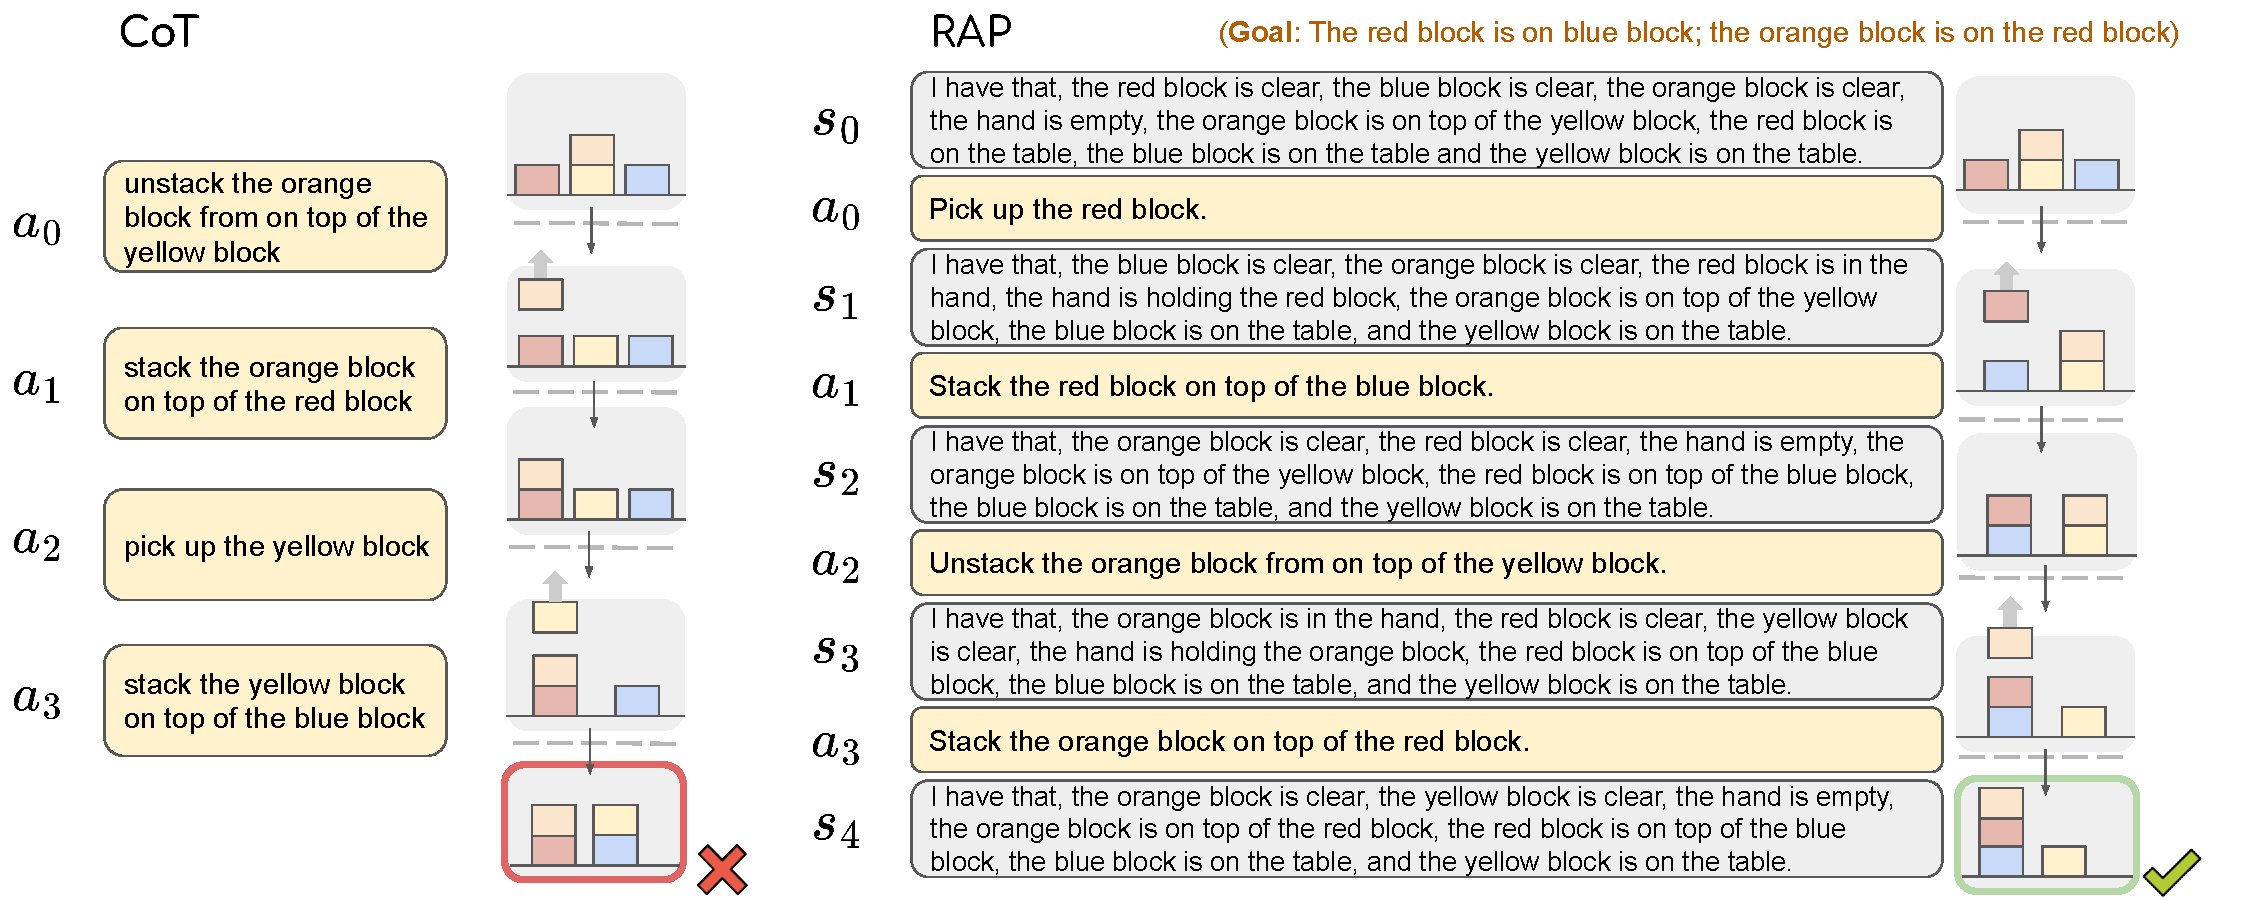
\includegraphics[width=0.9\textwidth]{sections/Figure-4_final.pdf}
    \vspace{-8pt}
    \caption{Comparing reasoning traces in \blocksworld from CoT (left) and \ours (right).}
    \label{fig:bw_example}
    \label{fig:my_label}
    \vspace{-12pt}
\end{figure*}



The plan generation task aims to produce a sequence of actions to achieve a given goal, possibly with additional constraints. The ability to generate plans is important for intelligent embodied agents, e.g. household robots~\cite{puig2018virtualhome}. % such as VirtualHome \cite{puig2018virtualhome} and \blocksworld \cite{valmeekam2022large}. 
% This task has also been widely used to evaluate the reasoning ability of LLMs given their challenging requirements of long-horizon reasoning, e.g., \blocksworld is a classic problem, where an agent is asked to rearrange the blocks into stacks in a particular order. 

% In these tasks, a plan is expected to be executable, meaning that each step in the plan must be valid when considering the conditions. \hsb{I feel that we don't need to emphasize the validity of actions, as that's not what we want to solve with RAP}
% In the \blocksworld domain where steps are actions that move blocks, an executable plan implies that each step is valid when considering the state of the blocks before the step (for instance, picking up a block is not allowed when there is already a block in the hand). 
% While not all plan generation tasks can be broken up into discrete steps, those that can provide a natural approach for adapting the RAP framework.
% what do we want to deliver with this sentence?
% As each step in a plan induces change in the current conditions, we formulate the set of conditions as the state of the world and individual steps as being state transitions.
%\hzt{Some of the discussions are too abstract. Perhaps use Blockworld as example.}

% \hzt{Need a figure to illustrate how the problem is mapped to our formulation. Refer to the figures in "Tree of Thoughts" in each experiment section.}

\noindent \textbf{Task setup.}
% \paragraph{Task setup.} 
To explore the viability of the RAP framework for plan generation tasks, we adapt and evaluate RAP on the \blocksworld benchmark~\cite{valmeekam2022large}, where an agent is asked to rearrange the blocks into stacks in a particular order. 
% This domain consists of a set of colored blocks that are either on top of a table or on top of another block. 
% With the goal being to reach an orientation of the blocks that satisfy some given conditions, the task is to rearrange the blocks with a series of valid actions. 
We define a \textbf{state} as the current orientation of the blocks and an \textbf{action} as an instruction that moves blocks. Specifically, an action is composed of one of the 4 verbs (i.e., \textsc{Stack}, \textsc{Unstack}, \textsc{Put}, and \textsc{Pickup}) and manipulated objects. For the action space, we generate the currently valid actions given the domain restrictions on actions and the current orientation of the blocks. To transit between states, we take the current action and query the LLM to predict the state changes to the relevant blocks. We then update the current state by adding the new block conditions and removing the conditions that are no longer true. Once a state has met all conditions in the goal or the depth limit of the tree is reached, we terminate the associated node.

To assess the quality of actions within this domain, we use two separate \textbf{rewards}. 
First, we prompt the LLM with some example test cases along with their solutions, and then calculate the log probability of the action given the current state (\textit{``Likelihood of action''} reward in Section~\ref{sec:reward}), denoted as $r_{1}$. This reward reflects the intuition of the LLM as the reasoning agent. It's typically indicative when there are few steps left to the goal, while not as reliable for a distant goal. Additionally, we compare the new state after performing an action with the goal and provide a reward, $r_{2}$, scaling with the number of conditions met (\textit{``Task-specific heuristics''} reward). Specifically, when all the conditions are met, we assign a super large reward to make sure this plan will be selected as the solution. %While there may be multiple plans that correctly reach the given goal, a given state usually has a clear action that is most optimal. Therefore, we do not apply 

%Aggregation \hsb{refer} doesn't apply to this task, because unlike ..., here all the reasoning steps will be included in the plan. 
%\hsb{can we specify the scope of aggregation in section 3? i.e. only available for result-oriented problems}
%on the search tree and instead find the reasoning trace with maximum reward when returning the final plan.



\begin{table}[t!]
    \small
    \centering
    % \vspace{pt}
    \begin{tabular}{r c c c}
        \toprule
        \textbf{Method} & \textbf{2-step} & \textbf{4-step} & \textbf{6-step}\\
        \midrule
        CoT & 0.17 & 0.02 & 0.00\\
        %\multicolumn{1}{r|}{ - pass@10} & 0.23 & 0.07 & 0.00 \\ 
        CoT - pass@10 & 0.23 & 0.07 & 0.00 \\ 
        %\multicolumn{1}{r|}{ - w/ GPT-4} 
        CoT (GPT-4) & 0.50  & 0.63 & 0.40\\
        
        \midrule
        RAP$^{(10)}$ & 1.00 & 0.86 & 0.26 \\
        RAP$^{(20)}$ & \textbf{1.00} & \textbf{0.88} & \textbf{0.42} \\
        \bottomrule
    \end{tabular}
    % \vspace{4pt}
    \vspace{-5pt}
    \caption{Results on \blocksworld. RAP$^{(10)}$ and RAP$^{(20)}$ refer to our method where the iteration number is set to 10 and 20, respectively. ``pass@10'' means 10 plans are sampled for each test case, and the test case is regarded as solved if at least one plan is correct. All other settings including RAP, only evaluate a single plan.}
    \label{tab:bw}
    \vspace{-12pt}
\end{table}


\noindent \textbf{Results.}
% \paragraph{Results.}
%We evaluate our framework on Blockworld, with the task being to generate a valid plan that reaches a goal given an initial state. 
We use test cases from the \blocksworld dataset \cite{valmeekam2023planning} and group them by minimum number of actions required, resulting in 30 cases solvable within 2 steps, 57 cases within 4 steps, and 114 cases within 6 steps.
% We also conduct experiments on the more challenging full Blocksworld with a stronger LLM in section \ref{sec:bw_appendix_full}.
There are at most 5 blocks in each test case. As the baseline method, we prompt the LLM with 4 test cases with corresponding solutions, and ask it to generate a plan for a new question. This setting is the same as one described in \citet{valmeekam2022large}, and we denote it as Chain-of-Thought (CoT) as the solution is generated step by step. For RAP, the same prompt is shown to help LLMs calculate $r_1$. 

As shown in Table~\ref{tab:bw}, CoT with LLaMA-33B can only generate successful plans for a few 2-step cases, and completely fails on harder problems. RAP substantially improves over CoT by nearly solving all problems within 4 steps, and a part of 6-step problems, achieving an average success rate of $64\%$. It's worth noting that the searching space of 6-step problems can be as large as $5^6$, while our algorithm can find a successful plan 42\% of the time within 20 iterations. Even more, our framework allows LLaMA-33B to outperform GPT-4 by $33\%$ relative gain, which is known to have much stronger reasoning ability~\cite{bubeck2023sparks}. %\footnote{For some unknown reasons, GPT-4 tends to generate long plans.}.


\noindent \textbf{Case study.}
We compare the reasoning paths from CoT and \ours in Figure~\ref{fig:bw_example}. We summarize the reasons accounting for the improvement: (1) By maintaining the world state during reasoning, RAP can recognize valid actions for the current state, avoiding generating illegal plans. (2) RAP is capable of backtracking and trying out other solutions when the first intuition from the LLM doesn't work. Specifically, CoT attempts to achieve the second goal, i.e. ``orange on red'', and achieve that with the first two steps. However, accomplishing the second goal first would prevent the first goal from being satisfied. On the contrary, even though RAP makes the same mistakes in the first iterations, our framework drives the agent to explore other possible paths (as described in Section~\ref{sec:mcts}) and finally generate a successful plan. (3) When calculating $r_t$, we can only feed the current state to the LLM and hide the history. E.g., in the case of Figure~\ref{fig:bw_example}, to calculate the reward for $a_2$, the LLM is provided with a ``new'' test case, in which $s_2$ is the initial state. This significantly lowers the difficulties of the last few steps, and saves more iterations for harder decisions of the first few steps.

%We take these instances from a dataset of problems that consist of a maximum of 5 blocks in each 
% shibo: I just checked the dataset and there are actually cases with 5 blocks.
%problem. With these instances, we further sort the problems based on the optimal number of steps needed to reach the goal. We use FILLER-shot examples for both our framework and the baselines, and do FILLER roll-outs in MCTS. \jjh{FILL will data + analysis}

% \vspace{-5pt}
\subsection{Math Reasoning} \label{sec:math}
% \vspace{-5pt}


\noindent \textbf{Task setup.}
% \paragraph{Task setup.} 
Math reasoning tasks, such as GSM8k \cite{cobbe2021training}, often include a description and a final question.
To arrive at the answer to the final question, it is necessary to undertake multi-step mathematical calculations 
%on the numbers provided in the description 
based on the problem's context.
It is thus natural to decompose the final question into a sequence of smaller sub-questions (Figure~\ref{fig:tree_examples}, right).
% \textcolor{blue}{
We define a \textbf{state} as the values of intermediate variables,
and an \textbf{action} as to propose an incremental sub-question about a unknown intermediate variable.
% To adapt RAP, we define a state as the already answered sub-questions \hzt{we shall say the state is the values of intermediate variables, and in implementation, instead of defining a new format, we simply stack all subquestions and their answers together to represent the state}, while an action is to propose a new sub-question.
The world model then responds to the sub-question using the intermediate variables and the problem description, adding the new intermediate variable value into the next state.
% For state transitions, the world model leverages the answers from previous sub-questions in the current state to respond to the new sub-question and incorporates it, along with its answer, into the next state \hzt{This sentence is long, a bit hard to understand.}.
% Furthermore, the world model assesses the quality of the newly proposed sub-question, serving as a reward for the action \hzt{reward is not part of WM}. 
% \hzt{The Method section has described several rewards. Refer to them, and describe new rewards if any.} We propose two evaluation methods.
We combine the self-evaluation of helpfulness by LLM $r_{t, 1}$ and the confidence of state $r_{t, 2}$ using weighted geometric mean $r_t = r_{t, 1}^\alpha * r_{t, 2}^{1 - \alpha}$ as the \textbf{reward} function.
% The first entails sampling the answer to the sub-question from the LLM and employing the confidence of the answer as the reward $r_{t, 1}$.
% This penalizes too difficult and jumping questions and encourages those future states with more reliable answers.
% The second involves querying the LLM with \texttt{Is the new question helpful?}, and using the probability of the token \texttt{Yes} as the reward $r_{t, 1}$.
% Since the calculation of $$
This reward encourages more relevant and useful sub-questions.
% We combine the two rewards using a weighted geometric mean, expressed as $r_t = r_{t, 1}^\alpha * r_{t, 2}^{1 - \alpha}$.
To account for the impact of the reasoning path's length on the reward, we compute \textbf{the $Q$ value} by using the maximum of average rewards in future steps.

\vspace{-5pt}
{
\small
\begin{align}
    Q^\ast (s_t, a_t) = \max_{s_t, a_t, r_t, \dots, s_l, a_l, r_l, s_{l+1}} \operatorname{avg}(r_t, \dots, r_l). 
    \label{eq:q-avg}
\end{align}
}
% }
% Since there may be multiple ways to decompose the final question, and the order of sub-questions may vary in correct reasoning paths, we apply the aggregation on the search tree to vote a answer across all roll-outs. \gy{describe scale by average length} \hzt{This paragraph is a bit long. Highlight (bolden) keywords like "reward", "state", "action" when we start defining them, to make the paragraph more structured.}

\begin{table}[t]
    \centering
    \small
    \begin{tabular}{r | c}
        %\vspace{-10em}
        \toprule
        \textbf{Method} & \textbf{Accuracy (\%)} \\
        \midrule
        Chain-of-Thought & 29.4 \\
        + SC$^{(10)}$ & 46.8 \\
        Least-to-Most & 25.5 \\
        + SC$^{(10)}$ & 42.5 \\
        \midrule
        RAP$^{(1)}$ & 40.0 \\
        RAP$^{(10)}$ & 48.6 \\
        + aggr & \textbf{51.6} \\
        \bottomrule
    \end{tabular}
    \vspace{-5pt}
    \caption{Results on GSM8k. The superscripts indicate the number of samples or iterations.}
    \vspace{-8pt}
    \label{tab:gsm8k}
\end{table}


% \begin{table}[t]
%     % \small
%     \centering
%     \begin{tabular}{r | c}
%         \toprule
%         \textbf{Method} & \textbf{Accuracy (\%)} \\
%         \midrule
%         Chain-of-thoughts & 29.4 \\
%         + SC$^{(10)}$ & 46.8 \\
%         Least-to-Most & 25.5 \\
%         + SC$^{(10)}$ & 42.5 \\
%         \midrule
%         RAP$^{(1)}$ & 40.0 \\
%         RAP$^{(10)}$ & 48.6 \\
%         + aggr & \textbf{51.6} \\
%         \bottomrule
%     \end{tabular}
%     \vspace{2pt}
%     \caption{GSM8k results.\hsb{add footnotes for comparison with llama paper}}
%     \label{tab:gsm8k}
% \end{table}

% \begin{figure}[t]
%     \centering
%     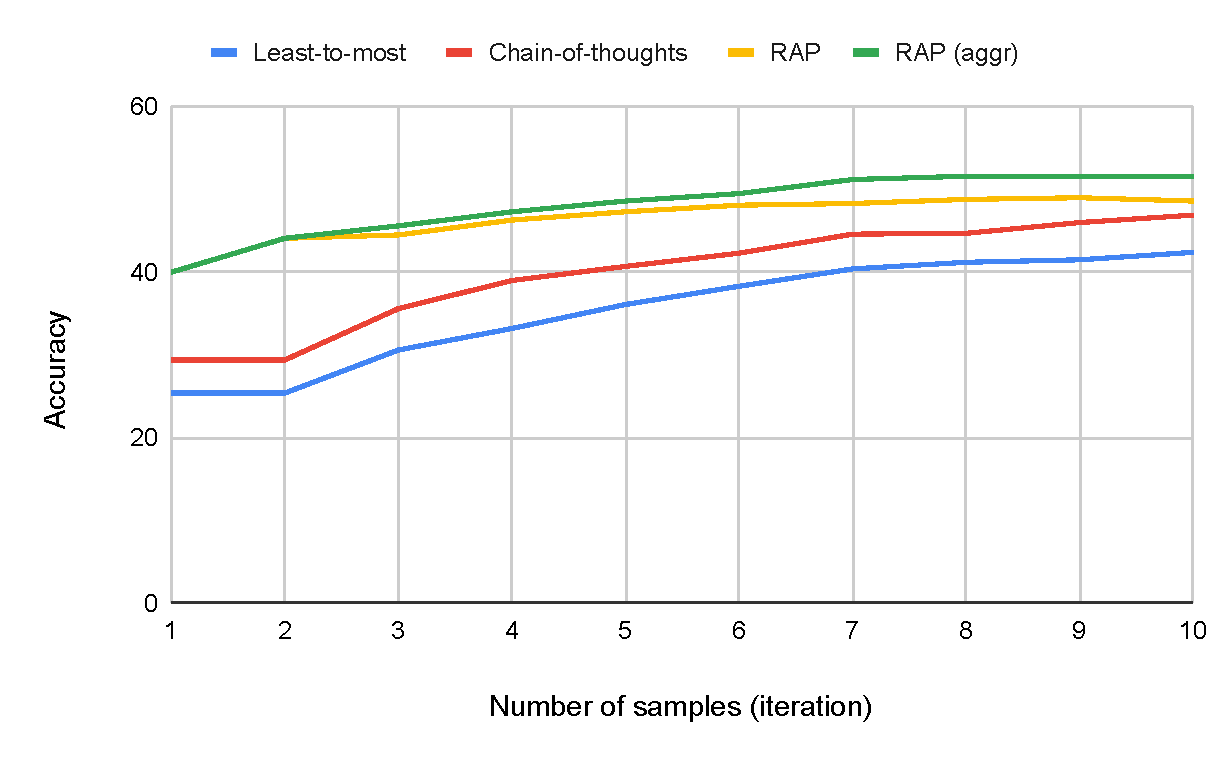
\includegraphics[width=\textwidth]{sections/chart.pdf}
%     %PLACEHOLDER \\
%     % \gy{Maybe we can put the table and figure side-by-side} It's ok to keep current format, fitting EMNLP's double-column format
%     \caption{\hsb{a figure (x-n\_samples, y-acc)}}
%     \label{fig:gsm8k-n_sample}
% \end{figure}

As a related work, Least-to-Most prompting \cite{zhou2022least} shares a similar idea to us in sub-question decomposition, but they generate sub-questions all at once. On the contrary, RAP considers each action $a_t$ based on the current state $s_t$, which enables more informed decisions.


\begin{figure}
\centering
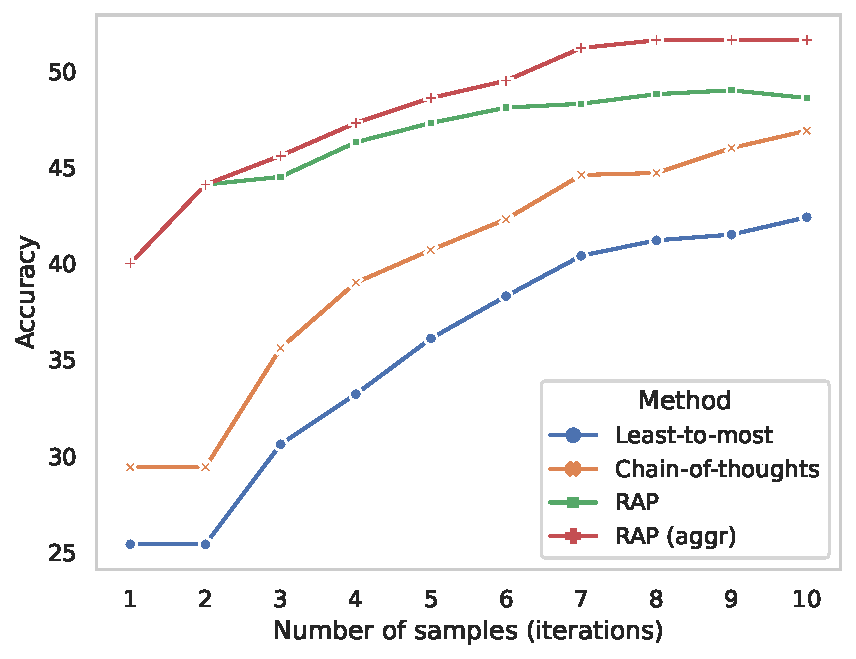
\includegraphics[width=0.8\linewidth]{sections/rap_results.pdf}
\vspace{-8pt}
\captionof{figure}{Results on GSM-8K, with different numbers of sampled paths or iterations.}
\label{fig:gsm8k-n_sample}
\vspace{-12pt}
\end{figure}




\noindent \textbf{Results.}
% \paragraph{Results.}
We evaluate our framework on GSM8k, a dataset of grade school math word problems. We also evaluate the base model with CoT prompting \cite{wei2022chain}, Least-to-Most prompting \cite{zhou2022least}, and their self-consistency \cite{wang2022self} variants, as the baselines. 
%\hzt{and self-consistency, please be complete}.
We use the same 4-shot examples demonstrations for all methods. % 10 iterations in MCTS and 10 samples in self-consistency baselines.
%\hzt{of baselines? Please be specific}.

As shown in Table \ref{tab:gsm8k}, our RAP framework answers $48.8\%$ of the problems correctly, outperforming both the Chain-of-Thought and the Least-to-Most prompting with Self-Consistency. Notably, this result is achieved when RAP only selects only one reasoning trace based on the reward.
The introduction of RAP-Aggregate further improves the accuracy by $\sim 3\%$.
We also calculate the accuracy with different numbers of iterations in MCTS and self-consistency samples in baselines, as illustrated in Figure \ref{fig:gsm8k-n_sample}.
We find that across all numbers of iterations/samples, \ours-Aggregation outperforms baselines consistently, which indicates that when only a few iterations/samples are allowed, our framework is significantly better at finding reliable reasoning paths with the guide of reward. 

\subsection{Logical Reasoning} \label{sec:logical}



\noindent \textbf{Task setup.}
% \paragraph{Task setup.}
% ProofWriter \cite{tafjord2020proofwriter}, FOLIO \cite{han2022folio}
%There exist many datasets for logical reasoning tasks, such as PrOntoQA \cite{saparov2022language}.
% In these datasets, one reasoning task typically comprises a set of facts and rules, along with a question presented a hypothesis fact to be determined true or false based solely on the given information.
A logical reasoning task (e.g. PrOntoQA \cite{saparov2022language}) typically provides a set of \emph{facts} and \emph{logical rules}, and a model is required to verify if a \emph{hypothesis fact} is true or false by applying the logical rules to the given facts, as illustrated in Figure \ref{fig:tree_examples}. These tasks not only require the correct final answer (true/false), but also a detailed proof demonstrating the result. To apply our framework, we define the \textbf{state} as a fact we are focusing on, analogous to the human's working memory~\cite{baddeley1992working} for inference. 
% \hzt{This is unclear, do you mean the pre-given set of facts, or also including the new facts derived during reasoning?}
An \textbf{action} is defined as selecting a rule from the fact set. The world model performs a one-hop reasoning step to get a new fact as the next state. The \textbf{reward} is calculated with Self-evaluation (Section~\ref{sec:reward}. Specifically, we prompt the LLM with a few examples with their labels to help it better understand the quality of reasoning steps.
% \hzt{the Method section does not use "state transition" much}.
% We also query the world model with the prompt \texttt{Is this reasoning step correct?}, \hzt{Reward is not part of world model.} and utilize the probability of the token \texttt{Yes} as the reward $r_t$.
We use the average reward of future steps to update \textbf{the $Q$ function}, the same as Equation (\ref{eq:q-avg}) for GSM8k.
% Among the logical reasoning datasets, PrOntoQA has a special characteristic in which each rule contains only one premise, resulting in a proof structured as a chain where only the new fact from the last step is required for each reasoning step.
% In such case, we can simplify our state design to be a single fact instead of a set of facts, and the state transition will involve employing the single fact and the proposed rule to perform a 1-hop reasoning and lead to the next state consisting of the new fact.
% We illustrate our world model's state and action definition in Figure \gy{figure}.


%\begin{figure}
%  \centering
%  % \vspace{-20pt}
%    \centering
%    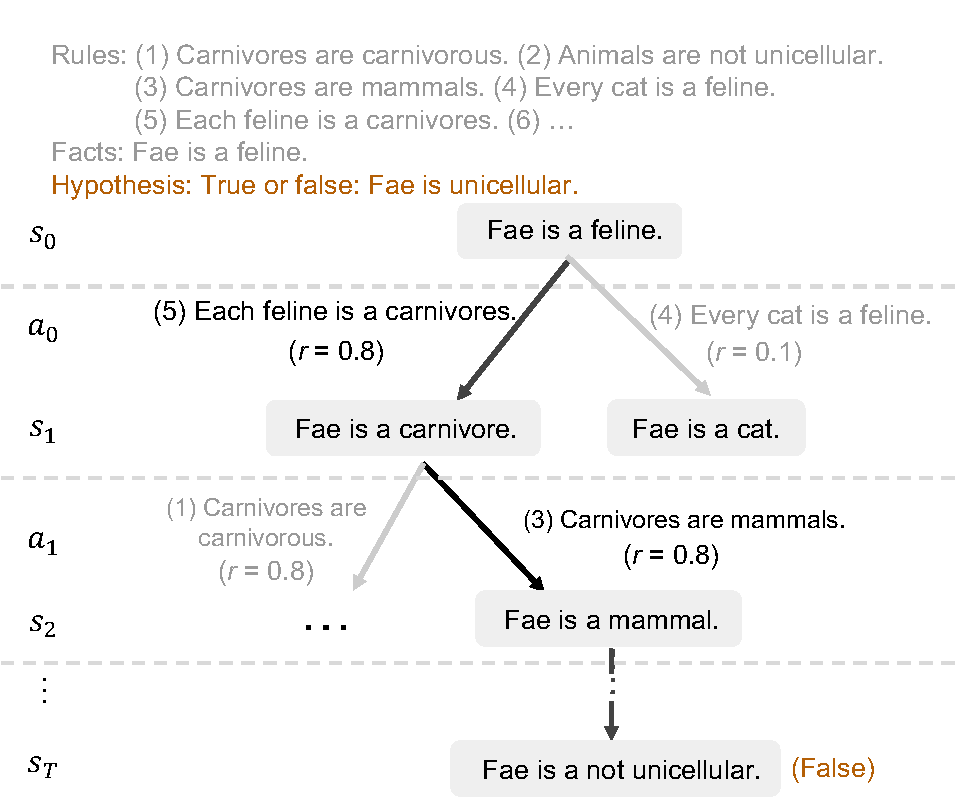
\includegraphics[scale=0.45]{sections/tree_logical.pdf}
%    \captionof{figure}{RAP planning on a PrOntoQA example.}
%    \label{fig:tree_logical}
%  \vspace{0pt}
%\end{figure}

\begin{table}
\centering
\small
\begin{tabular}{l c c}
    \toprule
    \textbf{Method} & \textbf{Pred Acc} & \textbf{Proof Acc} \\
    \midrule
    CoT & 87.8 & 64.8 \\
    CoT + SC & 89.8 & - \\
    \midrule
    RAP (Ours) & \textbf{94.2} & \textbf{78.8} \\
    \bottomrule
\end{tabular}
\vspace{-5pt}
\caption{Results on ProntoQA.}
\vspace{-15pt}
\label{tab:prontoqa}
\end{table}


\begin{table*}[ht!]
    \small
    \centering
    %\vspace{5pt}
    \begin{tabular}{c c c c c c c c c}
        \toprule
        \textbf{Setting} & \textbf{Method} & \textbf{2-step} & \textbf{4-step} & \textbf{6-step} & \textbf{8-step} & \textbf{10-step} & \textbf{12-step} & \textbf{All}\\
        \midrule
        Easy & CoT & 0.49 & 0.18 & 0.06 & 0.01 & 0.01 & 0.00 & 0.08\\
        & RAP$^{(10)}$ & 1.00 & 0.99 & 0.75 & 0.61 & 0.32& 0.32 & 0.65\\
        \midrule
        Hard & CoT & 0.22 & 0.14 & 0.02 & 0.02 & 0.00 & 0.00 & 0.05\\
        & RAP$^{(10)}$ & 0.67 & 0.76 & 0.74 & 0.48 & 0.17 & 0.09 & 0.51 \\
        \bottomrule
    \end{tabular}
    \vspace{-5pt}
    \caption{Results on the full \blocksworld with Llama-2 70B.}
    \label{tab:bw_full}
    \vspace{-15pt}
\end{table*}


\noindent \textbf{Results.}
% \paragraph{Results.}
We assess the performance of our RAP framework on PrOntoQA \cite{saparov2022language} and adopt their settings of ``true'' ontology (using real-world knowledge), ``random'' ordering of rules. We mix the examples requiring 3, 4, and 5 reasoning hops in a correct proof to prevent LLM from memorizing when to finish the reasoning. We sample 500 examples from the generation script released by \citet{saparov2022language}.
% \gy{not sure whether to mention (1) they only release the generation script, so we use that to generate 500 examples (2) intuition to mix 3, 4, 5-hop examples}
% We generate 500 examples by adhering to the dataset's ``true'' ontology, incorporating a mixture 3, 4 and 5-hop examples to discourage any potential exploitation of knowing when to finish the reasoning process
% \hzt{Cannot understand this sentence. Why do we "generate examples"? What does "adhering to the dataset's `true' ontology" mean? What does "3, 4 and 5-hop examples" mean? Also "discourage any potential exploitation of knowing when to finish the reasoning process" is hard to read}.
% We use chain-of-thought prompting \cite{wei2022chain} and its self-consistency \cite{wang2022self} variant as our baselines,
% \hzt{Self-consistency is another baseline --- We have two baselines. What we said here instead indicates we only have one baseline..}
We compare both the prediction accuracy of the final answer and the accuracy of the entire proof.
We do 20 iterations for MCTS and 20 samples for self-consistency.

As the results presented in Table \ref{tab:prontoqa}, our framework achieves a correct answer rate of 94.2\% and a proof accuracy of 78.8\%, surpassing the CoT baseline by 14\% proof accuracy and the self-consistency CoT baseline by $4.4\%$ prediction accuracy. Such substantial improvements clearly demonstrate the effectiveness of \ours in solving logical reasoning problems in PrOntoQA. Also, as the case illustrated in Figure~\ref{fig:tree_examples}, RAP can effectively recognize when a reasoning chain comes to a dead end, and propagate the signal back to earlier reasoning steps, with the planning algorithm allowing it to explore alternatives to the previous steps. The self-evaluation reward further helps RAP to recognize potential incorrect reasoning steps, encouraging the agent to avoid them in future iterations.

% Along with the self-evaluation reward, it informs the LLM of possible bad actions, and discourages further visits to this node.
% The self-evaluation helps RAP recognize the possible bad reasoning steps, discouraging further 
%\gy{why} \hzt{Does the original PrOntoQA paper report any results of other models like GPT3?}
